\documentclass{article}

\usepackage{standalone}
\usepackage{pgfplots}
\pgfplotsset{compat=newest}
\usepackage{tikz}
\usetikzlibrary{decorations.markings}
\usetikzlibrary{patterns}

\usepackage{subcaption}
\usepackage[margin=2.5cm]{geometry}
\usepackage{amsmath}
\usepackage{amssymb}


\newcommand\greybox[1]{
	\vskip\baselineskip
	\par\noindent\colorbox{lightgray}{
		\begin{minipage}{\textwidth}#1\end{minipage}
	}
	\vskip\baselineskip
}

\title{Forelesning 3}


\begin{document}
\maketitle


\section*{Den tidsuavhengige Schrödingerligningen}

Vi skal nå i dette kapitellet massere S.L. litt slik at vi den blir enklere å jobbe med framover.
Vi starter med å skille tids- og posisjons-avhengigeten fra hverandre.

\subsection*{Separasjon av variable}


Vi har S.L. som 
\begin{align}
 - \frac{\hbar^2}{2m}\frac{\partial^2 \Psi(x,t)}{\partial x^2} + V(x) \Psi(x,t) 
	= i\hbar \frac{\partial \Psi(x,t)}{\partial t} 
\end{align}
vi har allerede løst ligningen for tilfellet med $V(x)$, altså for en fri partikkel. Vi skal i 
det følgende løse S.L. for ikke trivielle potensialer.
Når vi antar (som vi nesten alltid gjør) at potensialet er tidsuavhengige ($V(x)=0$) 
så kan vi bruke separasjon av variabler til å løse ligningen. Dette er noe vi ofte gjør 
når vi kan skrive ligningen slik at all posisjons-avhengigeten til operatorene er på venstre og all 
tids-avhengigeten på høyre side av lighetstegnet.

Det gjøres ved å anta følgende Ansatz
\begin{align}
	 \Psi(x,t) = \psi(x)f(t)
\end{align}
dvs. vi antar at vi kan dekomponere bølgefunksjonen i en del som varierer som en funksjon av 
posisjon og en del som funksjon av tid.
Vi setter inn i S.L.
\begin{align}
 - \frac{\hbar^2}{2m}\frac{\partial^2}{\partial x^2} [\psi(x)f(t)] + V(x) \psi(x)f(t) 
	&= i\hbar \frac{\partial }{\partial t} [\psi(x)f(t)] \\
	\Rightarrow f(t)[-\frac{\hbar^2}{2m}\frac{\partial^2}{\partial x^2} \psi(x) + V(x) \psi(x)] 
	&= \psi(x) i\hbar \frac{\partial }{\partial t} f(t) \\
   \Rightarrow \frac{1}{\psi(x)} [-\frac{\hbar^2}{2m}\frac{\partial^2}{\partial x^2} \psi(x) 
   + V(x) \psi(x)] &= \frac{i\hbar}{f(t)}  \frac{\partial }{\partial t} f(t) \\
\end{align}
Vi har nå fått ligningen på en form slik at tids og posisjons-avhengigeten er på hver sin side av 
likhetstegnet. Den eneste måten at denne ligningen kan være oppfylt på helt generelt er om begge
sidene er lik en konstant. Vi kaller denne konstant $E$ siden vi skal assosiere den med partikkelens
energi, vi ser allerede at den må ha samme enhet som $V(x)$ som vi vet har enhet energi. Vi har  
\begin{align}
    \frac{1}{\psi(x)} [-\frac{\hbar^2}{2m}\frac{\partial^2}{\partial x^2} \psi(x) 
   + V(x) \psi(x)] = E
\end{align}
og 
\begin{align}
	   \frac{i\hbar}{f(t)}  \frac{\partial }{\partial t} f(t) = E
\end{align}
Den tidsavhengige ligningen er her veldig grei å løse og trengs bare å løse en gang for alle $V(x)$.
Vi har at 
\begin{align}
	 f(t) = f(0) e^{ -i \frac{Et}{\hbar} }
\end{align}
Vi absorberer $f(0)$ inn i $\psi(x)$, som vi normerer etterhvert uansett, og vi har at den tidsavhengige løsningen er 
\begin{align}
	 \Psi(x,t) = \psi(x)e^{-i \frac{Et}{\hbar}}
\end{align}
Så vi har nå redusert problemet til  å løse en ordinær differensialligning, hhilket er mye lettere 
enn partielle differensialligninger.
I tillegg har vi at 
\begin{align}
	 |\Psi(x,t)|^2 = |\psi(x)|^2
\end{align}
altså at sannsynlighetstettheten er tidsuavhengig hvis vi vet at systemet vårt er i tilstanden 
gitt av $\psi(x)$, og derfor kaller vi $\psi(x)$ stationære tilstander.


\section*{Partikkel i boks}
Vi skal nå beregne de stasjonære tilstandene for et spesifikt system, nemlig en såkalt 
partikkel i boks, som er bneskrevet av det følgende potensialet 
\begin{align}
	 V(x) = \begin{cases}
		0,  \hspace{.7cm} x \in (0, L) \\
		\infty,\hspace{0.5cm}  x \notin (0, L)
		\end{cases}
\end{align}
Vi kan forholdsvis enkelt løse S.L. for partikkelen inne i boksen, siden den her er
\begin{align}
	 - \frac{\hbar^2}{2m}\frac{\partial^2 }{\partial x^2} \psi(x) &= E\psi(x) 
	\hspace{1cm} x \in (0,L)\\
\Rightarrow \hspace{1cm}	 \frac{\partial^2 }{\partial x^2} \psi(x) &= -k^2\psi(x)
\end{align}
hvor vi introduserer konstanten $k=\frac{\sqrt{2mE}}{\hbar}$ og vi ser nå at 
bølgefunksjonen er like seg selv modulus en negativ konstant når 
den deriveres mhp. x to ganger, som vi vet er en egenskap cosinus og sinus kurver har. 
\begin{align}
	 \psi(x) = A \sin(kx) + B \cos(kx)
	\hspace{1cm} x \in (0,L)\\
\end{align}
Her er $A$ og  $B$ vilkårlige konstanter. Utenfor boksen så må vi ha at $\psi(x) = 0$, siden 
potensialet er uendelig her.
Videre så har vi at bølgefunksjonen må være kontinuerlig overalt siden T.U.S.L. er en 
andre-ordens ordinær differensialligning, fysikalsk betyr 
dette at sannsynligheten for å finne partikkelen ikke kan ha noen diskontinuiteter.
Spesifikt har vi da at 
\begin{align}
	 \psi(0) = A \sin(0) + B\cos(0) = B = 0
\end{align}
og 

\begin{align}
	 \psi(L) = A\sin(kL) = 0
\end{align}
Vi utelukker den trivielle løsninger med $A=0$ siden den representerer situasjonen med ingen 
partikkel i boksen. De andre mulige løsningene finner vi når sinus-funksjonen er 0, hvilket
er tilfellet når
\begin{align}
	 n\pi = kL \hspace{0.7cm} n = 1,2,3,...
\end{align}
Dette gir oss det diskrete sette av tillate verdier for $k$ som
\begin{align}
	 k_n = \frac{n\pi}{L}
\end{align}
Vi husker nå hvordan vi definerte variabelen $k$ og bruker det til å finne energien, som da  
også er kvantisert
\begin{align}
	 E_n = \frac{\hbar^2 k_n^2}{2m} = \frac{\hbar^2 n^2 \pi^2}{2 L^2 m}
\end{align}
Her har vi altså kvantiserte energi-nivåer.
Videre har vi bølgefunksjonen
\begin{align}
	 \psi(x) = A_n \sin( \frac{n\pi x}{L})
\end{align}
Vi kan bestemmer konstanten $A_n$ fra normaliseringskravet som 
\begin{align}
	1 &= \int_{-\infty}^{\infty} |\psi(x)|^2 dx \\
	  &= \int_{0}^{L} |A_n|^2 \sin^2( \frac{n\pi x}{L}) dx \\
	  &= |A_n|^2 \int_{0}^{L} \big( 1  - \cos( \frac{2n\pi x}{L}) \big) dx \\
	  &= |A_n|^2  \Big[ x  - \frac{L}{2n\pi} \sin( \frac{2n\pi x}{L}) \Big]_0^L dx \\
	  &= |A_n|^2  \frac{L}{2}
\end{align}
Vi velger nå fasen til amplituden til å være reel, hvilket gir oss konstanten som 
\begin{align}
	 A_n = \sqrt{ \frac{2}{L}}
\end{align}
For fullstendighetens skyld har vi nå hele den tidsuavhengige bølgefunksjonen som 
\begin{align}
	 \psi(x) = \begin{cases}
	\sqrt{\frac{2}{L}} \sin( \frac{n\pi x}{L}) \hspace{.7cm} x \in (0,L) \\
	 0				    \hspace{2.5cm} x \notin (0,L)
		\end{cases}
\end{align}
Dette er i sterk konstrant til det vi forventer av en klassisk partikkel i boks, siden klassisk
kan partikkelen ha alle mulige energier mens vi her har et diskret sett av mulige energinivåer.
Denne kvantiseringen kommer fra randbetingelsene, for den fullstendige frie partikkelen hadde 
vi ikke kvantiserte energinivåer.

I tillegg har vi at det ikke finnes noe $E=0$ løsning. Det kommer av at selv grunntilstanden 
oscillerer og beveger på seg.
Dette kan vi også se utifra Heisenberg's uskarphetsrelasjon. Hvis partikkelen hadde ingen energi 
hadde den ikke vært i bevegelse, altså vært helt i ro. Da ville bevegelsesmengden ha vært $0$
og dermed også $\Delta p =0$. Men det hadde da betydd at vi måtte ha hatt $\Delta x = \infty$
og det er ikke mulig siden vi vet med sikkerhet at partikkelen er inne i boksen.
Det er da også slik at for en mindre boks vil $\Delta x$ være mindre og $\Delta p$ derfor kunne 
være større, hvilket også tillater at energien er større.


\begin{figure}[h!]
     \centering
     \begin{subfigure}[b]{0.4\linewidth}
       \centering
	\begin{tikzpicture}
	  \begin{axis}%
	    [
	     xlabel=$x$,
	     ylabel=$y$,
	     axis lines=middle,
	     restrict y to domain=-2:2.,
	     enlargelimits={abs=.3}
	    ]
	    \addplot+[mark=none, 
		    domain=0:4,
		    samples=150,
		    draw=blue!70,
		    pattern color=blue,
	    	    area legend] {sin(deg(pi * x / 4)) * sqrt(2 / 4)}  ;
	    \node [above, color=blue!70] at (3, 0.75) {$\psi_1(x)$};
	  \end{axis}
	\end{tikzpicture}
         \label{fig:cos}
     \end{subfigure}
     \hspace{3cm}
     \begin{subfigure}[b]{0.4\linewidth}
         \centering
	\begin{tikzpicture}
	\begin{axis}%
	[
	xlabel=$x$,
	ylabel=$y$,
	axis lines=middle,
	restrict y to domain=-2:2.,
	enlargelimits={abs=.3}
	]
	\addplot+[mark=none, 
	    domain=0:4,
	    samples=350,
	    draw=red!70,
	    pattern color=blue,
	    area legend] {sin(deg(pi * x / 4))^2 * (2 / 4)}  ;
	    \node [above, color=red!70] at (3, 0.6) {$|\psi_1(x)|^2$};
	\end{axis}
	\end{tikzpicture}
         \label{fig:puls}
     \end{subfigure}
     \\
     \begin{subfigure}[b]{0.4\linewidth}
       \centering
	\begin{tikzpicture}
	  \begin{axis}%
	    [
	     xlabel=$x$,
	     ylabel=$y$,
	     axis lines=middle,
	     restrict y to domain=-2:2.,
	     enlargelimits={abs=.3}
	    ]
	    \addplot+[mark=none, 
		    domain=0:4,
		    samples=150,
		    draw=blue!70,
		    pattern color=blue,
	    	    area legend] {sin(deg(pi * x / 2)) * sqrt(2 / 4)}  ;
	    \node [above, color=blue!70] at (3, 0.75) {$\psi_2(x)$};
	  \end{axis}
	\end{tikzpicture}
         \label{fig:cos}
     \end{subfigure}
     \hspace{3cm}
     \begin{subfigure}[b]{0.4\linewidth}
         \centering
	\begin{tikzpicture}
	\begin{axis}%
	[
	xlabel=$x$,
	ylabel=$y$,
	axis lines=middle,
	restrict y to domain=-2:2.,
	enlargelimits={abs=.3}
	]
	\addplot+[mark=none, 
	    domain=0:4,
	    samples=350,
	    draw=red!70,
	    pattern color=blue,
	    area legend] {sin(deg(pi * x / 2))^2 * (2 / 4)}  ;
	    \node [above, color=red!70] at (3, 0.6) {$|\psi_2(x)|^2$};
	\end{axis}
	\end{tikzpicture}
         \label{fig:puls}
     \end{subfigure}
\\
     \begin{subfigure}[b]{0.4\linewidth}
       \centering
	\begin{tikzpicture}
	  \begin{axis}%
	    [
	     xlabel=$x$,
	     ylabel=$y$,
	     axis lines=middle,
	     restrict y to domain=-2:2.,
	     enlargelimits={abs=.3}
	    ]
	    \addplot+[mark=none, 
		    domain=0:4,
		    samples=150,
		    draw=blue!70,
		    pattern color=blue,
	    	    area legend] {sin(deg(pi * x * 3 / 4)) * sqrt(2 / 4)}  ;
	    \node [above, color=blue!70] at (3, 0.75) {$\psi_3(x)$};
	  \end{axis}
	\end{tikzpicture}
         \label{fig:cos}
     \end{subfigure}
     \hspace{3cm}
     \begin{subfigure}[b]{0.4\linewidth}
         \centering
	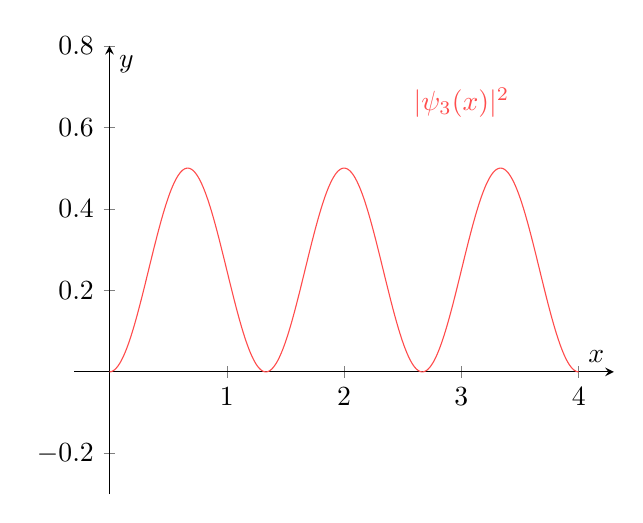
\begin{tikzpicture}
	\begin{axis}%
	[
	xlabel=$x$,
	ylabel=$y$,
	axis lines=middle,
	restrict y to domain=-2:2.,
	enlargelimits={abs=.3}
	]
	\addplot+[mark=none, 
	    domain=0:4,
	    samples=350,
	    draw=red!70,
	    pattern color=blue,
	    area legend] {sin(deg(pi * x * 3 / 4))^2 * (2 / 4)}  ;
	    \node [above, color=red!70] at (3, 0.6) {$|\psi_3(x)|^2$};
	\end{axis}
	\end{tikzpicture}
         \label{fig:puls}
     \end{subfigure}
        \caption{De tre første stasjonære tilstandene til partikkel i boks.}
        \label{fig:bølger}
\end{figure}

\subsubsection*{Tidsavhengighet}
Vi ser at om en partikkel er i en av de stasjonære tilstandene så er sannsynlighetstettheten
uavhengig av tid, og partikkelen beveger seg ikke. Partikkelen har ingen bestemt posisjon
men sannsynligheten for å finne partikkelen på forskjellige steder er konstant i tid.
Dette har vi siden 
\begin{align}
 \Psi_n(x,t) = \psi_n e^{-i \frac{E_nt}{\hbar}} \;\;\; \Rightarrow 
\;\;\; |\Psi_n(x,t)|^2 = |\psi_n(x)|^2
\end{align}
Hvis vi derimot ser for oss at partikkelen er i superposisjon av stasjonære tilstander, e.g. 
\begin{align}
	 \Psi(x, t) = \frac{1}{\sqrt{2}} \psi_1(x)  e^{-i \frac{E_1t}{\hbar}} 
	+ \frac{1}{\sqrt{2}}\psi_2(x)  e^{-i \frac{E_2t}{\hbar}}  
 \end{align}
 Da har vi 
 \begin{align}
	  |\Psi(x,t)|^2 &= (\frac{1}{\sqrt{2}} \psi_1(x)  e^{-i \frac{E_1t}{\hbar}} 
	+ \frac{1}{\sqrt{2}}\psi_2(x)  e^{-i \frac{E_2t}{\hbar}} ) 
	(\frac{1}{\sqrt{2}} \psi_1^*(x)  e^{i \frac{E_1t}{\hbar}} 
	+ \frac{1}{\sqrt{2}}\psi_2^*(x)  e^{i \frac{E_2t}{\hbar}}  ) \\
	&= \frac{1}{2} |\psi_1(x)|^2 + \frac{1}{2} |\psi_2(x)|^2   
	+ \frac{1}{2} \psi_1(x)\psi_2^*(x)  e^{i \frac{(E_2-E_1)t}{\hbar}} 
	+ \frac{1}{2} \psi_1^*(x)\psi_2(x)  e^{-i \frac{(E_2-E_1)t}{\hbar}}  \\
	&= \frac{1}{2} |\psi_1(x)|^2 + \frac{1}{2} |\psi_2(x)|^2   
	+ \psi_1(x)\psi_2(x)  \cos( \frac{(E_2-E_1)t}{\hbar})
 \end{align}
 hvor vi brukte at $\psi_n(x)$ er reel. Vi ser nå at for en partikkel som er i en blanding av 
 stasjonære tilstander så endrer sannsynlighetstettheten i tid, og partikkelens sannsynlighet 
 oscillerer fram å tilbake. Dette kommer av kryss-termene mellom $\psi_1$-leddet of 
 $\psi_2$-leddet, dette leder til en slags interferens mellom de forskjellige stasjonære 
 bøgefunskjonene.


 \section*{Statistisk tolkning av kvantemekanikk}
 Vi ser nå for oss en enda mer generell bølgefunksjon som en superposisjon av stasjonære
 tilstander som 
 \begin{align}
 	 \Psi(x,t) \sum_{n=1}^{\infty} c_n(t) \psi_n(x)
 \end{align}
hvor vi har $c_n(t) = c_n e^{-i \frac{E_n t}{\hbar}}$. 

Vi skal nå se at settet av alle stasjonære tilstander $\{\psi_n(x)\}$ utgjør 
et \textbf{ortonormalt sett}, dvs at de er ortogonale og normalisert. Dette er analogt med 
enhetsvektorene $ \mathbf{\hat{i}}_x$, $ \mathbf{\hat{i}}_y$ og $ \mathbf{\hat{i}}_z$ 
som vi kjenner fra $\mathbb{R}^3$, 
som vi vet er ortonormale mhp. et indreprodukt som vi kjenner som prikk-produktet. Dvs. vi har
\begin{align}
\mathbf{\hat{i}}_i \cdot \mathbf{\hat{i}}_j = \delta_{i,j}\hspace{0.5cm} \forall i,j \in [x, y, z]
\end{align}
hvor vi har Kroenecker-deltaet som 
\begin{align}
	 \delta_{n,m} = \begin{cases}
		1   \hspace{0.5cm} n = m \\
		0   \hspace{0.5cm} n \neq m
		\end{cases}
\end{align}
Her i $\mathbb{R}^3$ tolker vi ortogonaliteten til enhetsvektorene at de står vinkelrett 
på hverandre i rommet.

Tilsvarende har vi for de stasjonære tilstandene
\begin{align}
	\int_{-\infty}^{\infty} \psi^*_n(x)\psi_m(x) dx = 
	\delta_{n, m} \hspace{0.5cm} \forall n,m \in \mathbb{N}_+
\end{align}
Her har vi at indreprodukt ikke er prikk-produktet, men integralet over hele domenet av den 
ene bølgefunksjonen multiplisert med den kompleks konjugerte av den andre.
I tillegg er de stasjonære tilstandene $\psi_n$ \textbf{komplette},
dvs alle mulige tilstander (bølgefunksjoner) kan uttrykkes som en linearkombinasjon av de.
Altså kan alle mulige bølgefunksjoner skrives som
\begin{align}
	 \psi = \sum_{n=1}^{\infty} c_n\psi_n
\end{align}
Dette er i anologi med enhetsvektorene $ \mathbf{\hat{i}}_x$, $ \mathbf{\hat{i}}_y$ 
og $ \mathbf{\hat{i}}_z$,
hvor vi vet at enhver vektor i $\mathbb{R}^3$ kan skrives på formen 
\begin{align}
	\mathbf{v} = v_x \mathbf{\hat{i}}_x + v_y \mathbf{\hat{i}}_y + v_z \mathbf{\hat{i}}_z
\end{align}
hvor vi også kan finne vekten/komponenten til en av enhetsvektorene som
\begin{align}
v_i = \mathbf{\hat{i}}_i \cdot \mathbf{v} \hspace{0.5cm} \forall i,j \in [x, y, z]
\end{align}
altså ved å ta indreprodukt av vektoren med den vektoren i linearkombinasjon som vi vil finne 
vekten til.
Dette fungerer på samme måte for de stasjonære tilstandene, men vi har et annet indre produkt. 
Vi må her multiplisere bølgefunksjonen med den kompleks konjugerte av den stasjonære tilstanden 
som vi vil finne vekten til og integrere som 
\begin{align}
	 \int_{-\infty}^{\infty} \psi_n^* \psi \;dx
	&= \int_{-\infty}^{\infty} \psi_n^* \sum_{m=1}^{\infty} c_m \psi_m \;dx \\
	&= \sum_{m=1}^{\infty} c_m  \int_{-\infty}^{\infty} \psi_n^*\psi_m \;dx \\
	&= \sum_{m=1}^{\infty}   c_m \delta_{m, n}  \\
	&= c_n 
\end{align}
Koeffisientene $c_n$ spiller en veldig viktig rolle i kvantemekanikk, og vi har at for 
normaliserte bølgefunksjoner 
\begin{align}
  1 &= \int_{-\infty}^{\infty} |\psi|^2 dx \\
  &= \int_{-\infty}^{\infty}\sum_{m=1}^{\infty} c_m^*\psi^*_m \sum_{n=1}^{\infty} c_n\psi_n dx \\
  &= \sum_{m=1}^{\infty} \sum_{n=1}^{\infty} c_m^* c_n \int_{-\infty}^{\infty} \psi^*_m \psi_n dx\\
  &= \sum_{m=1}^{\infty} \sum_{n=1}^{\infty} c_m^* c_n \delta_{m,n} \\
  &= \sum_{m=1}^{\infty} |c_m|^2
\end{align}
hvor viser at kvadratet av koeffisientene summerer til en. Dette lokker på en tolkning av 
koeffisientene som sannsynligheter 
\begin{align}
	 |c_n|^2 = P_n
\end{align}
hvor de gir sannsynligheten for å måle at en partikkel har energien $E_n$ som er assosiert med 
den stasjonære tilstanden $\psi_n$.
Vi har da at de eneste tillatte verdiene vi kan måle for energien er $\{E_n\}$ og sannsynligheten 
for å måle $E_n$ er gitt som $|c_n|^2$, hvilket gir forventningsverdien som 
\begin{align}
	 \langle E \rangle = \sum_{n=1}^{\infty} |c_n|^2 E_n
\end{align}


\section*{Energi operatoren}

Vi betrakter ofte den tids S.L.
\begin{align}
	 ( - \frac{\hbar^2}{2m} \frac{\partial^2}{\partial x^2} + V(x) )\psi = E \psi
\end{align}
som en eigenverdi ligning. En eigenverdi-ligning er en hvor en operator virker på en funksjon 
gir en konstant multiplisert med funksjonen, slik som 
\begin{align}
	 \hat{O}f_{\lambda}(x) = \lambda f_{\lambda}(x)
\end{align}
hvor $ \lambda $ er eigenverdien til eigenfunksjonen $f_{\lambda}(x)$ til operatorene $ \hat{O} $. 
En operator er noe som virker på en funksjon og gir en ny funksjon.
Vi har sett implisitt sett posisjons operatoren $ \hat{x} = x$  allerede hvor vi har 
\begin{align}
	 \hat{x}\psi = x\psi
\end{align}
Vi har da at posisjons operatoren virker på bølgefunksjonen ved å multiplisere den med $x$.

Videre har vi bevegelsesmengde oepratoren $ \hat{p} = -i\hbar \frac{\partial}{\partial x}  $ 
Slik at vi har 
\begin{align}
	 \hat{p}\psi = \frac{\hbar}{i}\frac{\partial \psi}{\partial x} 
\end{align}
bevegelsesmengde operatoren virker på bølgefunksjonen ved å deriivere den mhp x og multiplisere 
med $-i\hbar$.
Vi kan nå se at planbølger med et bestemt bølgetall er eigenfunksjonen til $ \hat{p}$ siden vi 
har 
\begin{align}
 \hat{p} A e^{ikx} = A \frac{\hbar}{i} \frac{\partial}{\partial x}  e^{ikx} = \hbar k A e^{ikx} 
\end{align}
hvor vi ser at eigenverdien til planbølgen er $p_k = \hbar k$.

Vi kan nå se hvorfor T.I.S.L. er en eigenverdi-ligning. Vi vet at i ikke-relativistisk 
kvantemekanikk har vi at energien er summen av potensiell og kinetisk energi operatorene som 
\begin{align}
	 \hat{H} &= \frac{ \hat{p}^2}{2m} + V( \hat{x}) \\
	 &=  \frac{1}{2m}(\frac{\hbar}{i} \frac{\partial}{\partial x})^2 + V(x) \\
	 &=  -\frac{\hbar^2}{2m}\frac{\partial^2}{\partial x^2} + V(x) 
\end{align}
hvor vi kaller energi operatoren for \textbf{Hamilton operatoren} $ \hat{H} $.
Vi kan nå skrive T.I.S.L. som 
\begin{align}
	 \hat{H}\psi_n = E_n \psi_n
\end{align}
hvor vi har indeksert de forskjellige eigenfunksjonene med tilhørende eigenverdier med $n$.

Vi ser nå igjen på partikkel i boks og ser på en tilstand som er en superposisjon av de 
to første stasjonære tilstandene 
\begin{align}
	 \psi = c_1\psi_1 + c_2\psi_2
\end{align}
Vi lar Hamilton operatorene virke på denne tilstanden 
\begin{align}
	 \hat{H}\psi &= c_1 \hat{H}\psi_1 + c_2 \hat{H}\psi_2 \\
	 &= c_1 E_1\psi_1 + c_2 E_2\psi_2
\end{align}
siden vi vet at $\{\psi_n \}$ er eigentilstander til Hamilton operatoren, siden de løser S.L.
og vi har sett at S.L. kan skrives som Hamilton operatorens eigenverdi-ligning.
Vi kan nå finne forventningsverdien til energien 
\begin{align}
\int_{-\infty}^{\infty}	 \psi^*\hat{H}\psi dx 
&= \int_{-\infty}^{\infty} (c_1^*\psi_1^* + c_2^*\psi_2^*)  \hat{H} (c_1\psi_1 + c_2\psi_2)  dx \\ 
&= |c_1|^2 \int_{-\infty}^{\infty} \psi_1^*\hat{H} \psi_1 dx  
 + |c_2|^2 \int_{-\infty}^{\infty} \psi_2^*\hat{H} \psi_2 dx  
 + c_1^* c_2 \int_{-\infty}^{\infty} \psi_1^*\hat{H} \psi_2 dx  
 + c_2^*c_1 \int_{-\infty}^{\infty} \psi_2^*\hat{H} \psi_1 dx  \\
&= |c_1|^2 E_1 \int_{-\infty}^{\infty}  |\psi_1|^2 dx  
 + |c_2|^2 E_2 \int_{-\infty}^{\infty}  |\psi_2|^2 dx  
 + c_1^* c_2 E_2 \int_{-\infty}^{\infty}  \psi_1^* \psi_2 dx  
 + c_2^*c_1 E_1 \int_{-\infty}^{\infty}  \psi_2^*\psi_1 dx  \\
&= |c_1|^2 E_1 + |c_2|^2 E_2
\end{align}
Vi sa at vi tolker $|c_n|^2$ som sannsynligheten for å måle $E_n$ så vi ser da at vi må ha 
\begin{align}
	 \langle E \rangle  = \int_{-\infty}^{\infty} \psi^* \hat{H} \psi dx
\end{align}
Dette gjelder også generelt at vi har forventningsverdien til enhver variabel 
\begin{align}
	 \langle O \rangle =  \int_{-\infty}^{\infty} \psi^* \hat{O} \psi dx
\end{align}
og vi har ellerede sett at dette stemmer for posisjon og bevegelsesmengden.

\end{document}
